\documentclass{article}

\usepackage{amsmath}
\usepackage{amssymb}
\usepackage{amsthm}
\usepackage{caption}
\usepackage{changepage}
\usepackage{fancyhdr}
\usepackage[margin=0.8in]{geometry}
\usepackage{graphicx}
\usepackage{tikz}
\usepackage{titlesec}

\pagestyle{fancy}

\lhead{Ryan Gibson}
\rhead{Linux Page Fault Experiment} 

\setlength\parindent{0pt}
\pagenumbering{gobble}

\begin{document}
\vspace*{-40pt}
\section{Procedure}
	We wrote a simple kernel module to provide statistics about the page faults of a Linux process.\\
	
	In particular, we kept track of the virtual and physical addresses associated with each page fault and the amount of time required for each page fault handler to execute.\\
	
	This was achieved by overriding the page fault handlers for each virtual memory area and adding the required logging code before and after calling the original fault handler.\\
	
	We then observed the page faulting behavior on various patterns of file access on a solid state drive.
\section{Data and Observations}
	All experiments were run after a complete boot of the system\footnote{Both host and virtual machine were rebooted.} (to completely clear OS page caches; to have a ``cold cache'') and with as few background processes running as possible (to minimize CPU or I/O interference from other processes).\\
	
	Each experiment involves repeatedly accessing a 45 MB file, one byte at a time (approximately 45 million accesses over 11300 4KB pages), while doing some very minor computation. Only page faults associated with this file will be considered (i.e. we will ignore any other faults, e.g. those associated with the text of our program).\\
	
	In these experiments, we will differentiate between page faults that require disk access (here, referred to as ``disk faults'') and those that do not (``non-disk faults''). If in the page fault handler, the desired page is not associated with a physical page frame (\texttt{vmf->page == NULL}), we know this particular fault reads the file from disk into the OS page cache.\\
	
	It's important to note that a page fault requiring disk access will be immediately followed by one only retrieving from the OS page cache since writing a page into the cache and mapping the page into page tables are handled separately. The latter page faults take less than 1 microsecond to handle and it will sometimes be useful to exclude them in our analysis.\\
	
	Hence, we will use the term ``short non-disk fault'' for these quick faults associated with mapping into page tables and ``long non-disk fault'' for those faults not associated with disk operation at all.

\subsection{Random File Access}

	First, we logged the page fault behavior when accessing our $\sim$45 MB file completely randomly.
	
	\begin{figure}[ht!]
		\centering
		\begin{tabular}{|c|c|c|c|c|}
			\cline{3-4}\multicolumn{2}{}{}&\multicolumn{2}{|c|}{Non-disk faults}\\
			\hline & Disk faults & Short & Long & All faults\\\hline
			Count & 6198 & 6198 & 5101 & 17497\\
			Percentage & 35\% & 35\% & 29\% & 100\% \\
			Average Fault Cost ($\mu$s) & 147.9 & 0.3 & 6.5 & 54.4\\
			Total Fault Cost (ms)\footnotemark[2] & 916.9 & 1.8 & 33.3 & 952.0 \\\hline
		\end{tabular}
		\caption{Page fault statistics for random file access. Note only 6198 memory accesses (about 0.01\%)\textsuperscript{3} required use of the disk even though we used all 11300 pages of the file.}
	\end{figure}
	\footnotetext[2]{``Fault Cost'' is the execution time of the page fault handler, excluding any overhead induced by our logging and behavior tracking.}
	\footnotetext[3]{6198 disk faults out of about 45 million file accesses is approximately 0.01\%.}
	\begin{figure}[ht!]
		\centering
		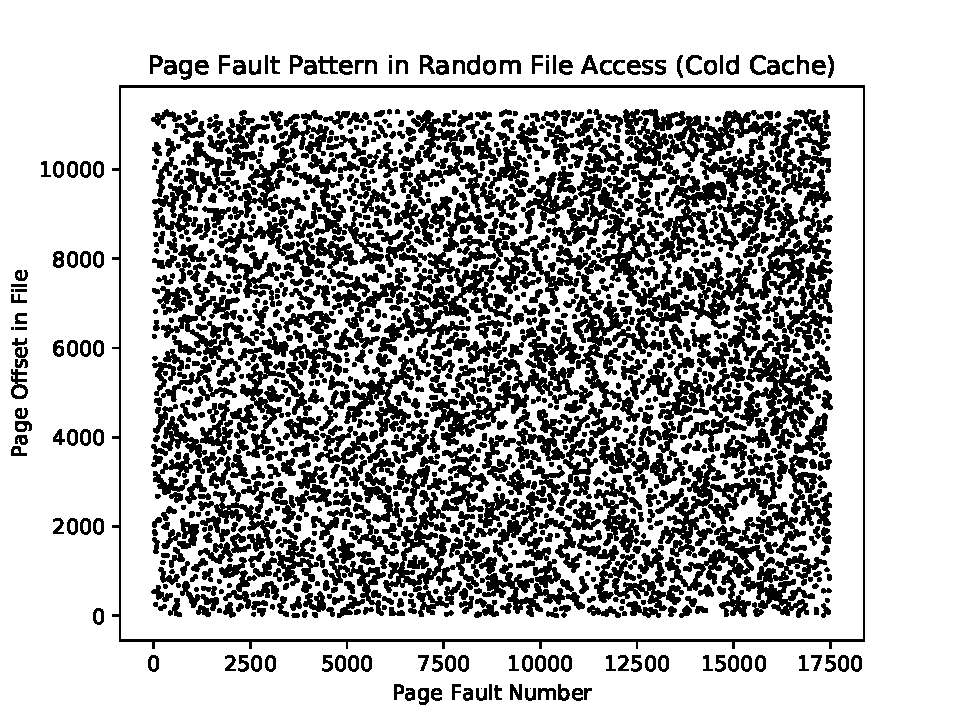
\includegraphics[width=0.45\linewidth, trim=0.4cm 0.4cm 0.4cm 0.4cm]{figures/random1.pdf}
		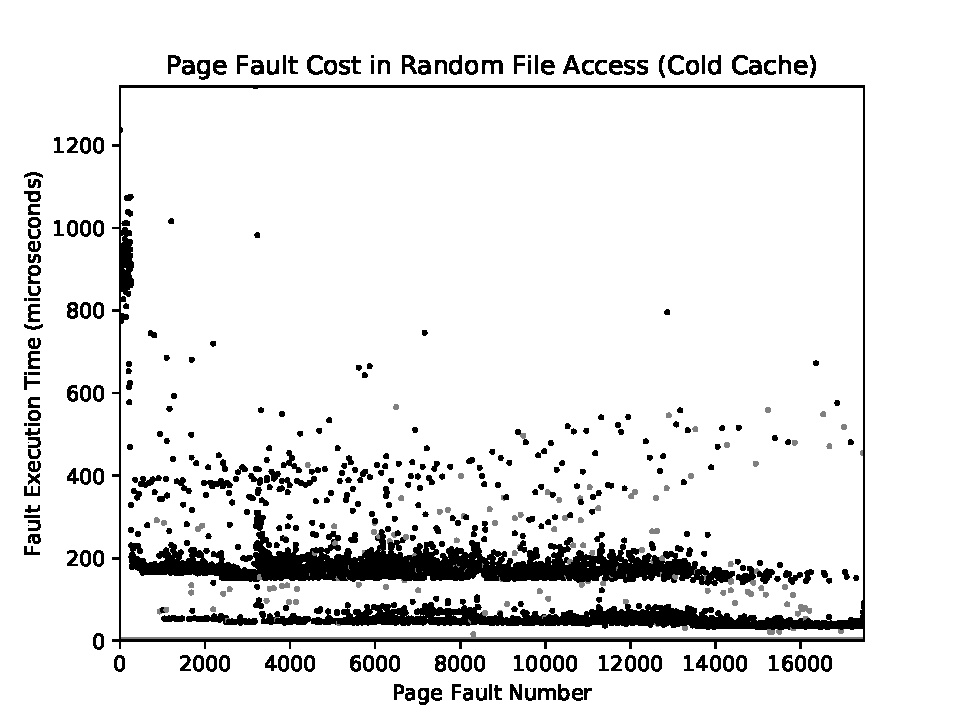
\includegraphics[width=0.45\linewidth, trim=0.4cm 0.4cm 0.4cm 0.4cm]{figures/random2.pdf}
		\caption{Left: the order of page faults in our random file access. Right: the page fault costs throughout the experiment. Disk faults are shown in black and non-disk faults are shown in gray. Note that all short non-disks faults are clustered on the $x$-axis (due to their fast operation).}
	\end{figure}
	
	It's interesting to note that the initial disk fault cost is high (near 1000 $\mu$s) before it alternates between about $200 \mu$s and $\sim$$50\mu$s (with $50\mu$s becoming increasingly common as the experiment progresses).\\
	
	As seen in \texttt{blockdev --report} (as root), our virtual machine has an SSD readahead of 256 blocks, each of size 4 KB. Hence, when possible, the disk will attempt to prepage 1 MB ahead of the current memory access.\\
	
	I believe that this attempt at prepaging is the main cause of the initial high disk fault cost (especially since $1000\mu$s is significantly higher than the disk's advertised access time / ``seek time'').\\
	
	However, the eventual disk fault cost of $\sim$$50 \mu$s is below the disk's advertised access time! I believe that the SSD controller is copying the file to the disk's DRAM cache as it ``realizes'' that the file of interest is being frequently accessed. This is further supported by the fact that $\sim$$50 \mu$s is a fairly typical access latency for commodity DRAM.\\
	
	For the sake of completeness, we now present the same experiment, but with the file already in OS page caches / buffers (``warm cache'').
	
	\begin{figure}[ht!]
		\centering
		\begin{tabular}{|c|c|c|c|c|}
			\cline{3-4}\multicolumn{2}{}{}&\multicolumn{2}{|c|}{Non-disk faults}\\
			\hline & Disk faults & Short & Long & All faults\\\hline
			Count & 0 & 0 & 9412 & 9412\\
			Percentage & 0\% & 0\% & 100\% & 100\% \\
			Average Fault Cost ($\mu$s) & - & - & 0.14 & 0.14\\
			Total Fault Cost (ms) & 0.0 & 0.0 & 1.3 & 1.3 \\\hline
		\end{tabular}
		\caption{Page fault statistics for random file access with a warm cache.}
	\end{figure}\vspace*{-20pt}
	\begin{figure}[ht!]
		\centering
		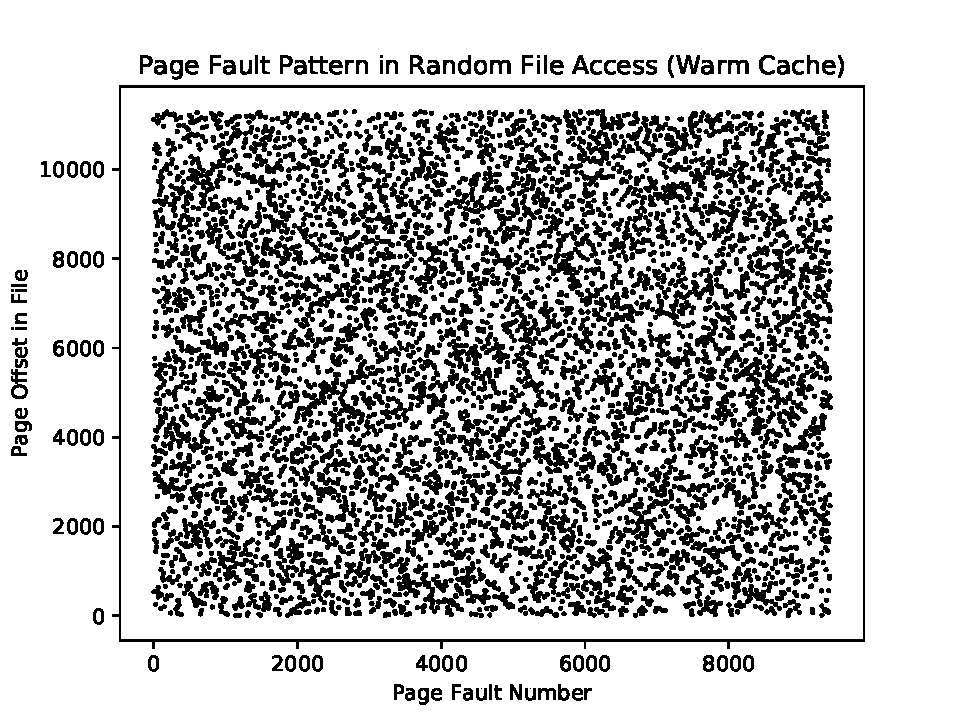
\includegraphics[width=0.43\linewidth, trim=0cm 0.4cm 0.4cm 0.4cm]{figures/warmrandom1.pdf}
		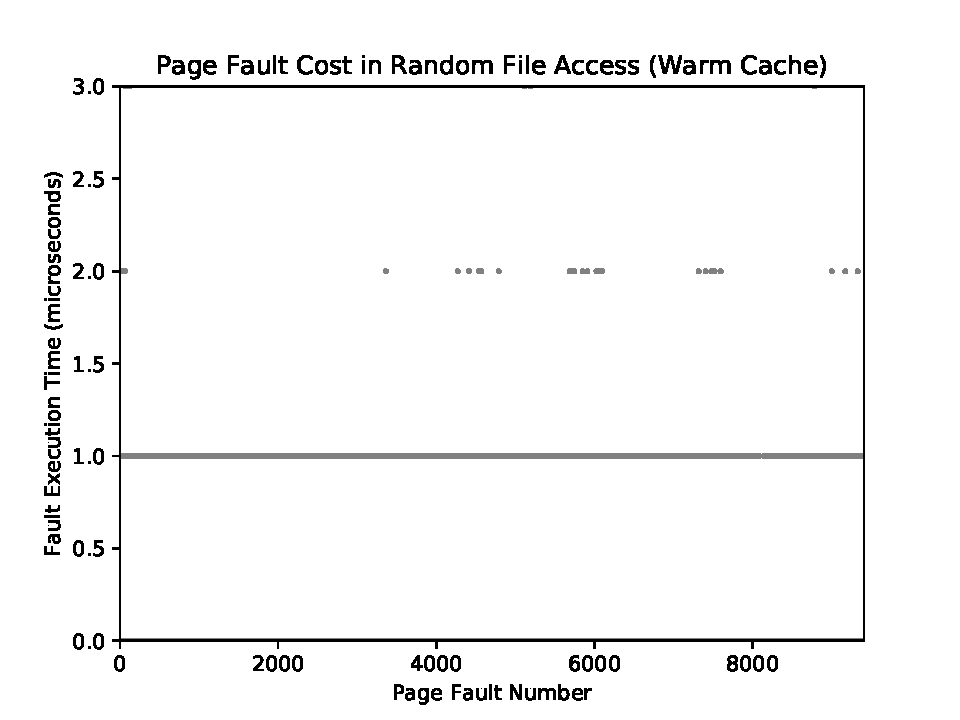
\includegraphics[width=0.43\linewidth, trim=0cm 0.4cm 0.4cm 0.4cm]{figures/warmrandom2.pdf}
		\caption{Left: the order of page faults in our random file access with a warm cache. Right: the page fault costs throughout the experiment. Disk faults are shown in black and non-disk faults are shown in gray.}
	\end{figure}
	
	Unsurprisingly, our long non-disk faults now behave as the short non-disk faults did with a cold cache since the relevant pages are already in OS buffers.\\
	
	The other experiments have similarly uninteresting results with a warm cache and will be omitted.
		
\subsection{Sequential File Access}

	Next, we logged the page fault behavior when accessing our $\sim$45 MB file in sequential byte order.
	\begin{figure}[ht!]
		\centering
		\begin{tabular}{|c|c|c|c|c|}
			\cline{3-4}\multicolumn{2}{}{}&\multicolumn{2}{|c|}{Non-disk faults}\\
			\hline & Disk faults & Short & Long & All faults\\\hline
			Count & 1 & 1 & 11299 & 11301\\
			Percentage & 0\% & 0\% & 100\% & 100\% \\
			Average Fault Cost ($\mu$s) & 1647.0 & 1.0 & 2.0 & 2.1 \\
			Total Fault Cost (ms) & 1.6 & 0.0 & 22.2 & 23.8 \\\hline
		\end{tabular}
		\caption{Page fault statistics for sequential file access.}
	\end{figure}
	
	\begin{figure}[ht!]
		\centering
		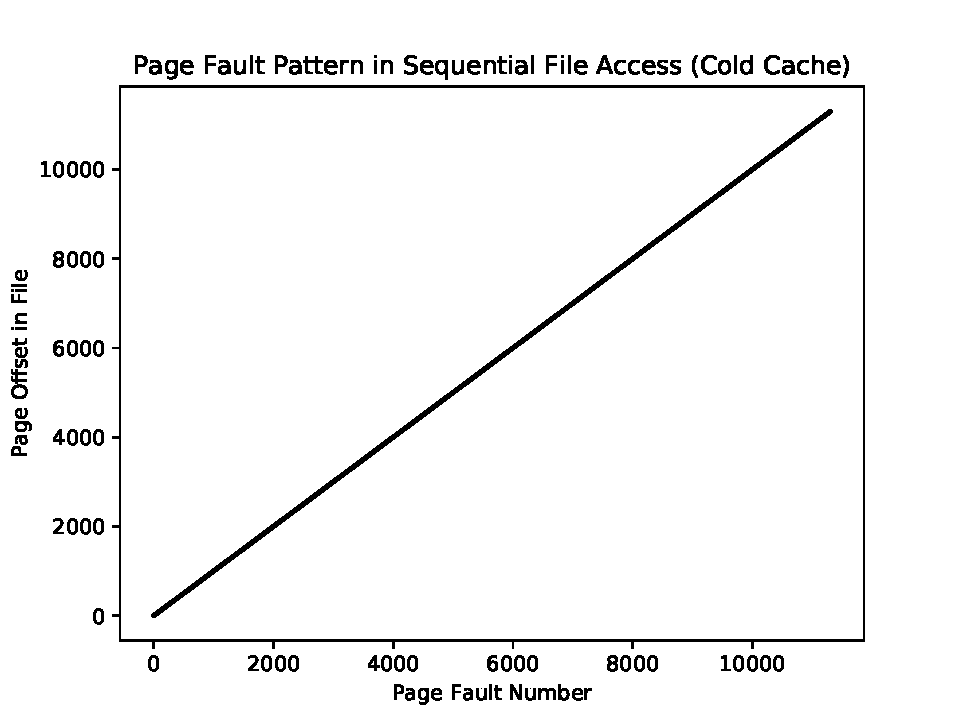
\includegraphics[width=0.45\linewidth, trim=0.4cm 0.4cm 0.4cm 0.4cm]{figures/sequential1.pdf}
		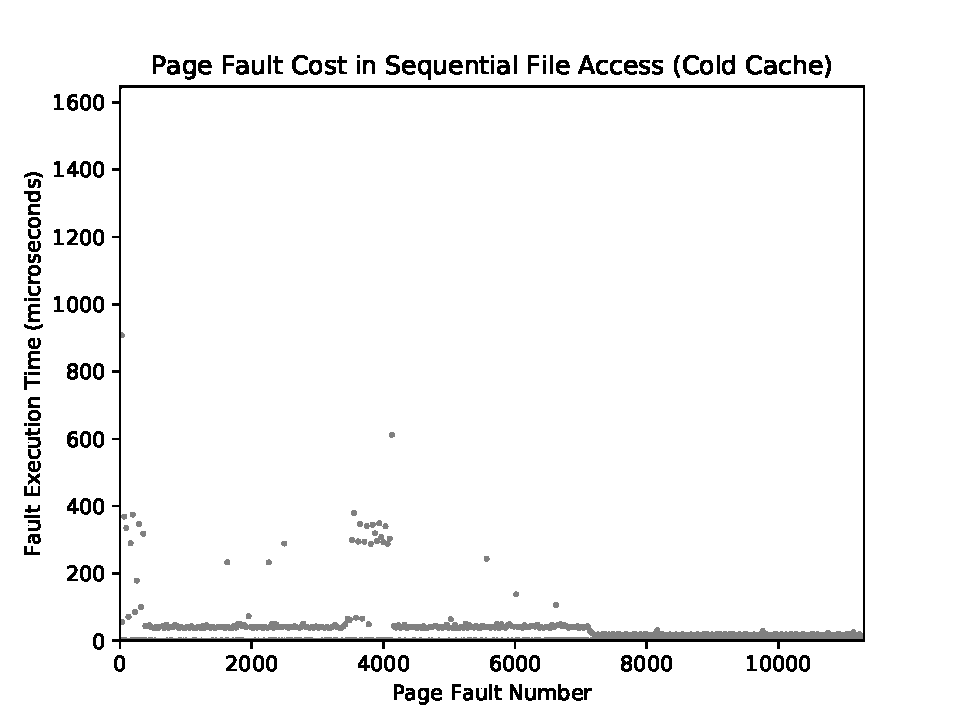
\includegraphics[width=0.45\linewidth, trim=0.4cm 0.4cm 0.4cm 0.4cm]{figures/sequential2.pdf}
		\caption{Left: the order of page faults in our sequential file access. Right: the page fault costs throughout the experiment. Disk faults are shown in black and non-disk faults are shown in gray.}
	\end{figure}
	
	Note that we have exactly one disk fault in this experiment! Only the first memory access of the file actually requires disk access in the page fault handler.\\
	
	Recalling that our SSD has a readahead of 1 MB, I believe that the disk is capable of perpetually looking ahead far enough for the purposes of our program here.

\subsection{Striding File Access}

	Next, we logged the page fault behavior when accessing our $\sim$45 MB file in a ``stride'' of 4096 bytes (1 page) per memory access (i.e. the page trace is $0, 1, 2, 3, \dots$). We still access 45 million bytes in this experiment.
	
	\begin{figure}[ht!]
		\centering
		\begin{tabular}{|c|c|c|c|c|}
			\cline{3-4}\multicolumn{2}{}{}&\multicolumn{2}{|c|}{Non-disk faults}\\
			\hline & Disk faults & Short & Long & All faults\\\hline
			Count & 58 & 58 & 11242 & 11358\\
			Percentage & 0.5\% & 0.5\% & 99\% & 100\% \\
			Average Fault Cost ($\mu$s) & 270.2 & 0.2 & 1.8 & 3.1 \\
			Total Fault Cost (ms) & 15.7 & 0.0 & 19.7 & 35.4 \\\hline
		\end{tabular}
		\caption{Page fault statistics for 4 KB striding file access.}
	\end{figure}
	\begin{figure}[ht!]
		\centering
		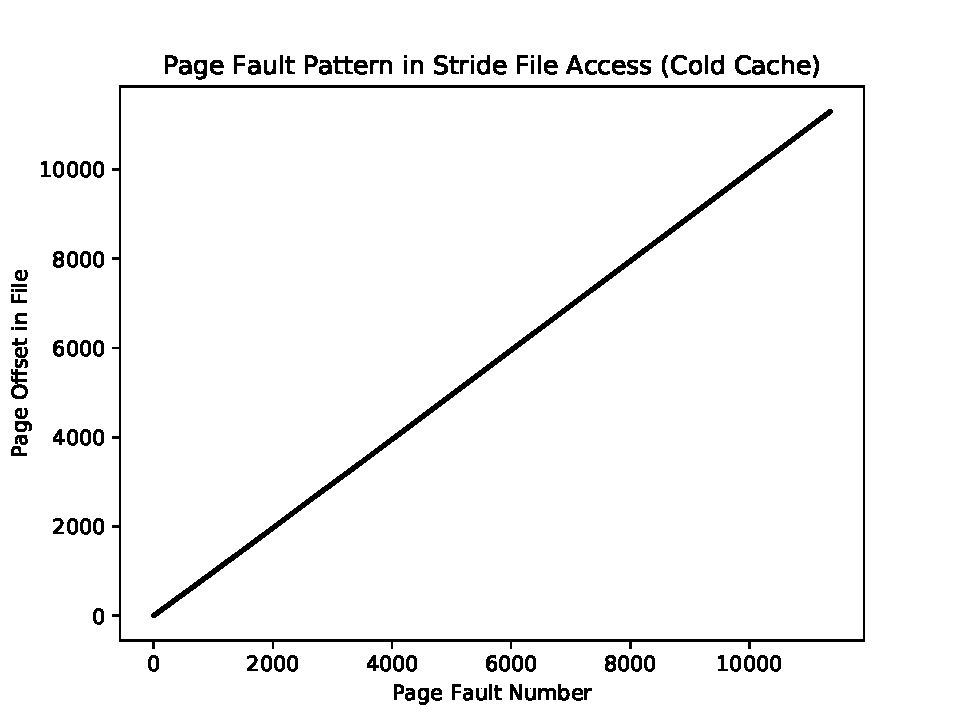
\includegraphics[width=0.45\linewidth, trim=0.4cm 0.4cm 0.4cm 0.4cm]{figures/stride1.pdf}
		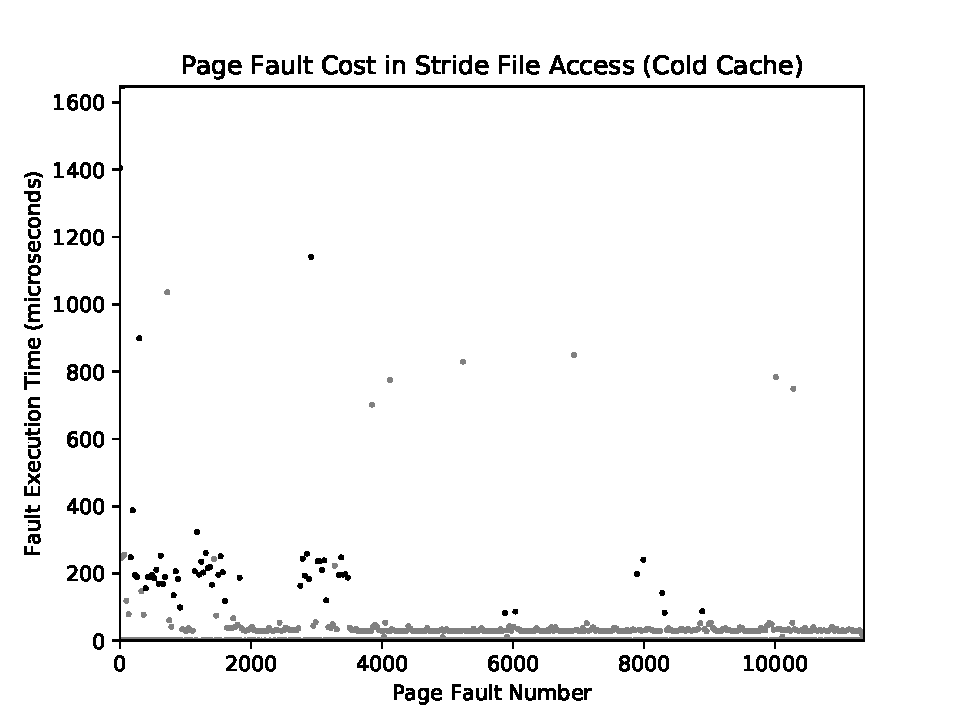
\includegraphics[width=0.45\linewidth, trim=0.4cm 0.4cm 0.4cm 0.4cm]{figures/stride2.pdf}
		\caption{Left: the order of page faults in our 4 KB striding file access. Right: the page fault costs throughout the experiment. Disk faults are shown in black and non-disk faults are shown in gray.}
	\end{figure}
	
	Note that even though we stride across the file 4096 times (to maintain 45 million memory accesses), we only page fault on the first sweep of the file. On later sweeps, we already have the relevant pages in memory.\\
	
	Here, the disk faults are clustered together around page fault 1000 and page fault 3000. Once again, I believe that the SSD manages to readahead enough to satisfy page faults $\sim$2000-3000 and either eventually moves most of the relevant file into its DRAM cache and/or reads far enough ahead for the purposes of our program afterwards (hence the relative lack of disk page faults from number 4000 onwards).\\
		
	A natural follow-up question is ``what happens if we stride faster than this readahead?''\\
	
	As such, we next logged the page fault behavior when accessing our $\sim$45 MB file in a stride of $64 \cdot 4096 = 256$ KB so that our page trace skips ahead 64 pages on each memory access. We still access 45 million bytes in this experiment.
	
	\vspace*{-10pt}
	\begin{figure}[ht!]
		\centering
		\begin{tabular}{|c|c|c|c|c|}
			\cline{3-4}\multicolumn{2}{}{}&\multicolumn{2}{|c|}{Non-disk faults}\\
			\hline & Disk faults & Short & Long & All faults\\\hline
			Count & 7224 & 7224 & 4075 & 18523\\
			Percentage & 39\% & 39\% & 22\% & 100\% \\
			Average Fault Cost ($\mu$s) & 115.3 & 0.2 & 4.4 & 46.0 \\
			Total Fault Cost (ms) & 833.0 & 1.8 & 17.8 & 852.6 \\\hline			
		\end{tabular}
		\caption{Page fault statistics for 256 KB striding file access.}
	\end{figure}\vspace*{-18pt}
	\begin{figure}[ht!]
		\centering
		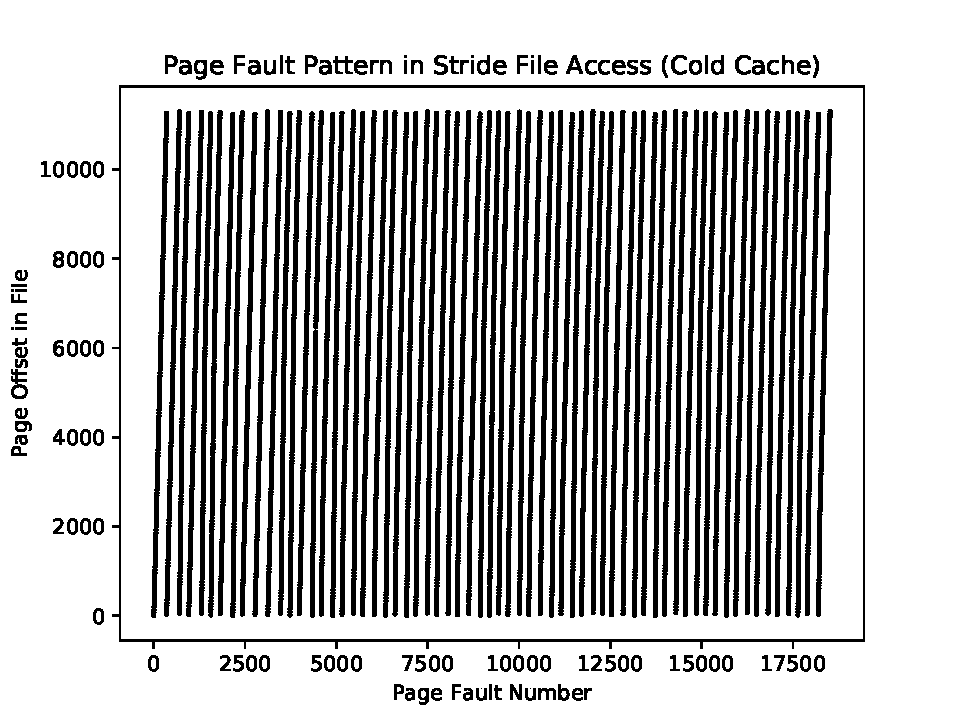
\includegraphics[width=0.45\linewidth, trim=0.4cm 0.4cm 0.4cm 0.4cm]{figures/longstride1.pdf}
		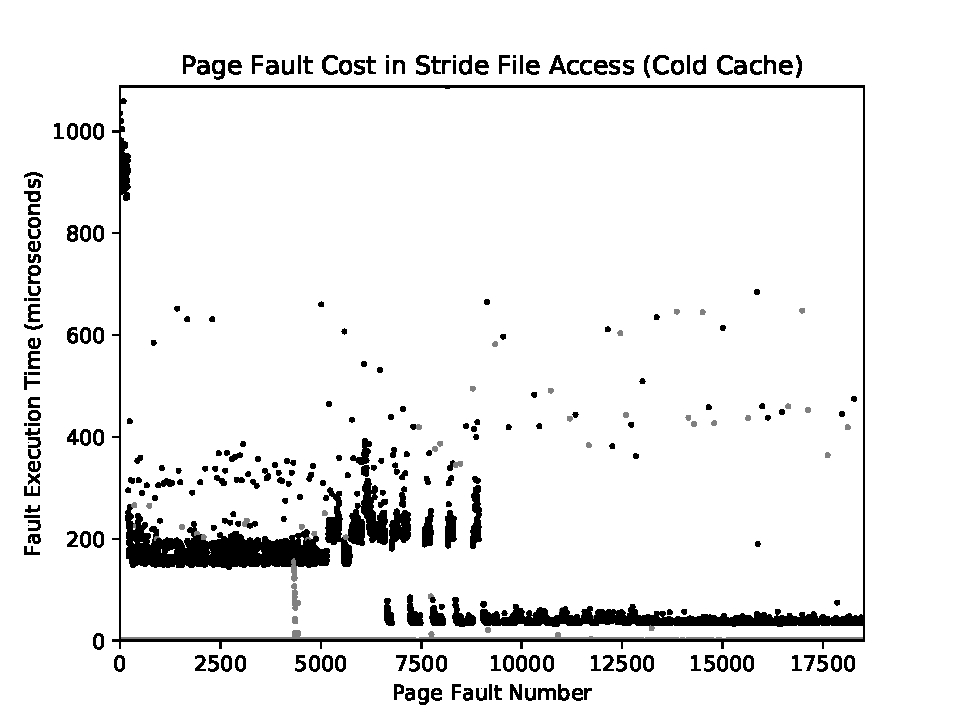
\includegraphics[width=0.45\linewidth, trim=0.4cm 0.4cm 0.4cm 0.4cm]{figures/longstride2.pdf}
		\caption{Left: the order of page faults in our 256 KB striding file access. Right: the page fault costs throughout the experiment. Disk faults are shown in black and non-disk faults are shown in gray.}
	\end{figure}
	
	Once again, note that we only have 64 sweeps of page faults until the entire file is stored in memory (since each sweep loads 1/64th of the file due to our stride length of 64 pages). On later sweeps, the relevant pages are already in memory.\\
	
	Further note that we are certainly striding faster than the drives readahead speed as our performance has degraded nearly to that of random file access.\\
	
	As always, we can see the disk fault cost move from $\sim$$200 \mu$s to $\sim$$50 \mu$s when the SSD (supposedly) transfers most of the file to its DRAM cache.\\
	
	I believe the rapid alternation between these two disk fault costs around page fault 6000 to 9000 is due to the memory accesses quickly striding through parts of the file not yet copied to this DRAM cache.
	
\section{Conclusions}

	Page fault analysis (and thus, some disk benchmarking) is easily achieved through use of our kernel module.\\

	Demand paging as seen in Linux appears extremely effective in ``normal use cases'' (with an SSD, at least). In a sequential read of a file, we only saw the process waiting for disk access at the very start of the program. This type of read is one of the most common for a ``typical'' user and is well optimized (both by the disk hardware and the OS prepaging capabilities).\\
	
	Even when striding across the file much more rapidly than a typical program, we saw an increase in total fault cost by about 50\% (see Figure 5 vs. Figure 7).\\
	
	In fact, the use of the disk no longer appears to be as extreme of a bottleneck as it once was as long as we purposefully exploit these disk and Linux optimizations in our programs (i.e. staying far away from the absurdity of random file access -- locality should be maintained if at all possible).
\end{document}